
%(BEGIN_QUESTION)
% Copyright 2011, Tony R. Kuphaldt, released under the Creative Commons Attribution License (v 1.0)
% This means you may do almost anything with this work of mine, so long as you give me proper credit

Dette enkle reguleringssystemet har et problem: trykket vist på regulatorens front viser nøyaktig setpunkt (95 tommer vannsøyle), men trykkmåleren stemmer ikke.

$$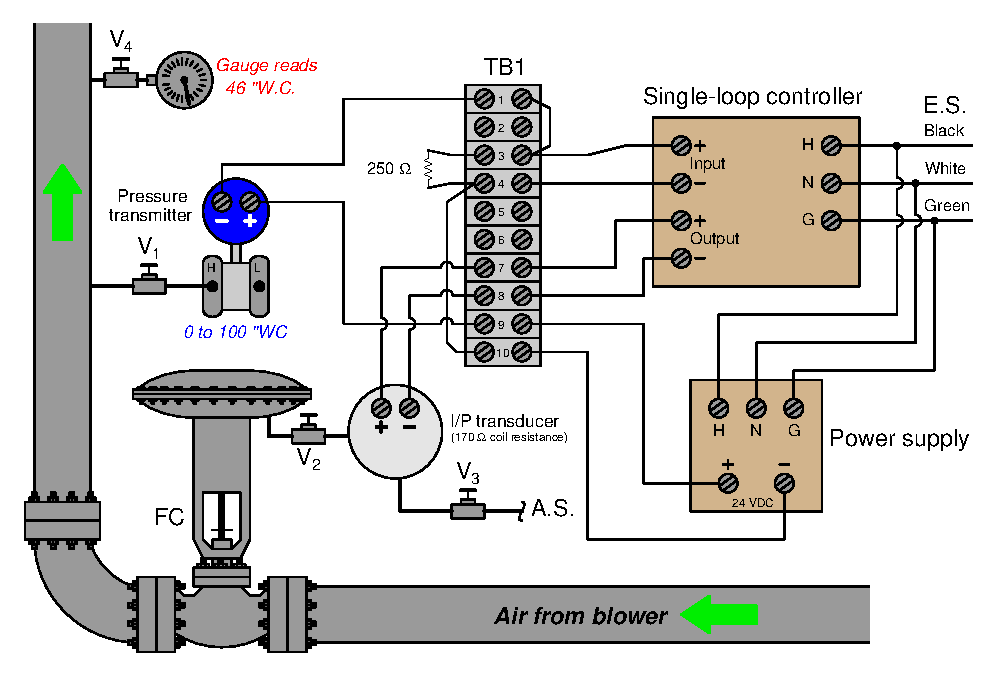
\includegraphics[width=15.5cm]{i00583x01.eps}$$

Vurder den diagnostiske verdien av hver test under. Anta kun én feil i systemet, enten i én komponent eller i én enkel leder/kabel/slange mellom komponenter. Hvis en test kan gi ny informasjon som hjelper deg å identifisere lokasjon og/eller type feil, marker ``ja''. Hvis ikke, marker ``nei''.

% No blank lines allowed between lines of an \halign structure!
% I use comments (%) instead, so that TeX doesn't choke.

$$\vbox{\offinterlineskip
\halign{\strut
\vrule \quad\hfil # \ \hfil & 
\vrule \quad\hfil # \ \hfil & 
\vrule \quad\hfil # \ \hfil \vrule \cr
\noalign{\hrule}
%
% First row
{\bf Diagnostisk test} & {\bf Ja} & {\bf Nei} \cr
%
\noalign{\hrule}
%
% Another row
Mål AC-nettspenning &  &  \cr
%
\noalign{\hrule}
%
% Another row
Mål DC-utgang fra strømforsyning &  &  \cr
%
\noalign{\hrule}
%
% Another row
Inspiser PID-parametere i regulator &  &  \cr
%
\noalign{\hrule}
%
% Another row
Kontroller kalibrering av trykktransmitter &  &  \cr
%
\noalign{\hrule}
%
% Another row
Mål transmitterens strømsignal &  &  \cr
%
\noalign{\hrule}
%
% Another row
Sett regulator i manuell og flytt ventil &  &  \cr
%
\noalign{\hrule}
%
% Another row
Mål DC-spenning mellom TB1-3 og TB1-4 &  &  \cr
%
\noalign{\hrule}
%
% Another row
Mål DC-spenning mellom TB1-7 og TB1-8 &  &  \cr
%
\noalign{\hrule}
} % End of \halign 
}$$ % End of \vbox


\underbar{file i00583}
%(END_QUESTION)





%(BEGIN_ANSWER)

\noindent
{\bf Delvis svar:}

% No blank lines allowed between lines of an \halign structure!
% I use comments (%) instead, so that TeX doesn't choke.

$$\vbox{\offinterlineskip
\halign{\strut
\vrule \quad\hfil # \ \hfil & 
\vrule \quad\hfil # \ \hfil & 
\vrule \quad\hfil # \ \hfil \vrule \cr
\noalign{\hrule}
%
% First row
{\bf Diagnostisk test} & {\bf Ja} & {\bf Nei} \cr
%
\noalign{\hrule}
%
% Another row
Mål AC-nettspenning &  & $\surd$ \cr
%
\noalign{\hrule}
%
% Another row
Mål DC-utgang fra strømforsyning &  & $\surd$ \cr
%
\noalign{\hrule}
%
% Another row
Inspiser PID-parametere i regulator &  &  \cr
%
\noalign{\hrule}
%
% Another row
Kontroller kalibrering av trykktransmitter &  &  \cr
%
\noalign{\hrule}
%
% Another row
Mål transmitterens strømsignal & $\surd$ &  \cr
%
\noalign{\hrule}
%
% Another row
Sett regulator i manuell og flytt ventil &  &  \cr
%
\noalign{\hrule}
%
% Another row
Mål DC-spenning mellom TB1-3 og TB1-4 & $\surd$ &  \cr
%
\noalign{\hrule}
%
% Another row
Mål DC-spenning mellom TB1-7 og TB1-8 &  &  \cr
%
\noalign{\hrule}
} % End of \halign 
}$$ % End of \vbox

Å flytte ventilen i manuell modus er nyttig {\it bare} dersom du samtidig observerer både måler- og regulatorindikasjon ved ny ventilposisjon. Begge bør endre seg når ventilposisjonen endres.

%(END_ANSWER)





%(BEGIN_NOTES)

% No blank lines allowed between lines of an \halign structure!
% I use comments (%) instead, so that TeX doesn't choke.

$$\vbox{\offinterlineskip
\halign{\strut
\vrule \quad\hfil # \ \hfil & 
\vrule \quad\hfil # \ \hfil & 
\vrule \quad\hfil # \ \hfil \vrule \cr
\noalign{\hrule}
%
% First row
{\bf Diagnostisk test} & {\bf Ja} & {\bf Nei} \cr
%
\noalign{\hrule}
%
% Another row
Mål AC-nettspenning &  & $\surd$ \cr
%
\noalign{\hrule}
%
% Another row
Mål DC-utgang fra strømforsyning &  & $\surd$ \cr
%
\noalign{\hrule}
%
% Another row
Inspiser PID-parametere i regulator &  & $\surd$ \cr
%
\noalign{\hrule}
%
% Another row
Kontroller kalibrering av trykktransmitter & $\surd$ &  \cr
%
\noalign{\hrule}
%
% Another row
Mål transmitterens strømsignal & $\surd$ &  \cr
%
\noalign{\hrule}
%
% Another row
Sett regulator i manuell og flytt ventil & $\surd$ &  \cr
%
\noalign{\hrule}
%
% Another row
Mål DC-spenning mellom TB1-3 og TB1-4 & $\surd$ &  \cr
%
\noalign{\hrule}
%
% Another row
Mål DC-spenning mellom TB1-7 og TB1-8 &  & $\surd$ \cr
%
\noalign{\hrule}
} % End of \halign 
}$$ % End of \vbox

At måleren og regulatoren er uenige om trykket forteller at feilen enten ligger i måleren, eller i signalveien transmitter-regulator. Verken tuning, strømforsyning eller ventil kan alene gi dette symptomet. Nyttige tester er derfor de som skiller mellom feil i måler, transmitter, motstand eller regulatorens PV-inngang.

%INDEX% Feilsøking, repetisjon: nytte av diagnostiske tester i elektriske kretser

%(END_NOTES)

